% ICRA submission. Official class from PaperCept (ieeeconf.zip).
% 8 pages INCLUDING references. Double-anonymous review.
%
% Status: DRAFT. Every number in Sections IV-V is measured and reproducible
% from the scripts named in the captions. Section VI (real vehicle) is not
% done and is marked as such rather than written speculatively.
\documentclass[letterpaper, 10 pt, conference]{ieeeconf}
\IEEEoverridecommandlockouts
\overrideIEEEmargins

\usepackage{graphicx}
\usepackage{amsmath,amssymb}
\usepackage{booktabs}
\usepackage{siunitx}
\usepackage{subcaption}
\usepackage{tikz}
\usepackage[hidelinks]{hyperref}
\usetikzlibrary{arrows.meta,positioning,shapes.geometric,calc,fit,backgrounds}

\sisetup{detect-weight=true, detect-family=true}

\title{\LARGE\bf Differentiating a Real-Time MPC Is Safe:\\
A Measurement, and the Test That Says Otherwise}

\author{Anonymous submission%
\thanks{Double-anonymous review; author and funding information removed.}}

\begin{document}
\maketitle
\thispagestyle{empty}
\pagestyle{empty}

\begin{abstract}
Treating a model-predictive controller as a differentiable function of its cost
weights underpins a growing family of methods that tune those weights online.
The gradient they use rests on the envelope theorem, which is exact \emph{at a
solution}. Deployed controllers are not at a solution: they run a fixed, small
number of SQP steps per tick and warm-start from the previous one, which makes
them formally recurrent --- the warm start is hidden state --- so their
sensitivity to the cost weights contains a term the envelope theorem cannot
see. We set out to measure that term and find that \textbf{it does not matter}.
For a genuine real-time iteration the memoryless gradient is exact in direction
(cosine $1.0000$) and $16\%$ off in magnitude, which for a method whose step
size is a tuned hyperparameter is not a distinction. The assumption the
literature makes without stating it is therefore justified, and this is the
measurement that justifies it. We also report the test that appears to refute
it: approximating real-time iteration by capping an interior-point solver at
one iteration yields a gradient orthogonal to the memoryless one, not because
of solver memory but because none of those solves converge --- the iterate
moves an order of magnitude further than a converged step. Separately, we show
that an online tuner needs a predictive safety filter to survive its own
learning ($0$ crashes in $26$ episodes against $8/8$ without, and nine times
the distance covered), and that the filter converts a catastrophic failure into
a slow one rather than removing it.
\end{abstract}

\section{Introduction}

\todo{One paragraph on why online cost tuning is attractive for racing: the
weights are few, interpretable, and the thing that actually decides lap time.}

The contributions are:
\begin{enumerate}
  \item the observation that a warm-started, iteration-limited MPC is
        formally a recurrent system, and the corresponding influence recursion
        (Section~\ref{sec:theory});
  \item a measurement showing the term that recursion adds is negligible for
        real-time iteration, so that the standard memoryless gradient is
        justified (Section~\ref{sec:rti});
  \item a methodological warning: the natural way to test this --- capping an
        interior-point solver's iterations --- inverts the answer, for a reason
        that is easy to miss (Section~\ref{sec:trap});
  \item the failure mode of unconstrained online tuning, and a predictive
        safety filter that removes it (Section~\ref{sec:safety});
  \item an open implementation of seven safety filters on one interface, with
        the measurement that the choice of \emph{criterion} matters far less
        than the model each is given.
\end{enumerate}

\section{Related work}

\todo{Gros \& Zanon (MPC as function approximator); mpcrl / MPC4RL; COAT-MPC
and Bayesian tuning; AD-MPCC; Diehl's RTI; Wabersich \& Zeilinger predictive
safety filters; Ames et al.\ CBFs; Gurriet \& Ames ASIF.}

The point of departure is that every method in the first group differentiates
\emph{through a solution}. None states the convergence of the deployed solver
as an assumption, and Section~\ref{sec:rti} shows it is one.

\section{MPCC and the two errors}

\begin{figure}[t]
  \centering
  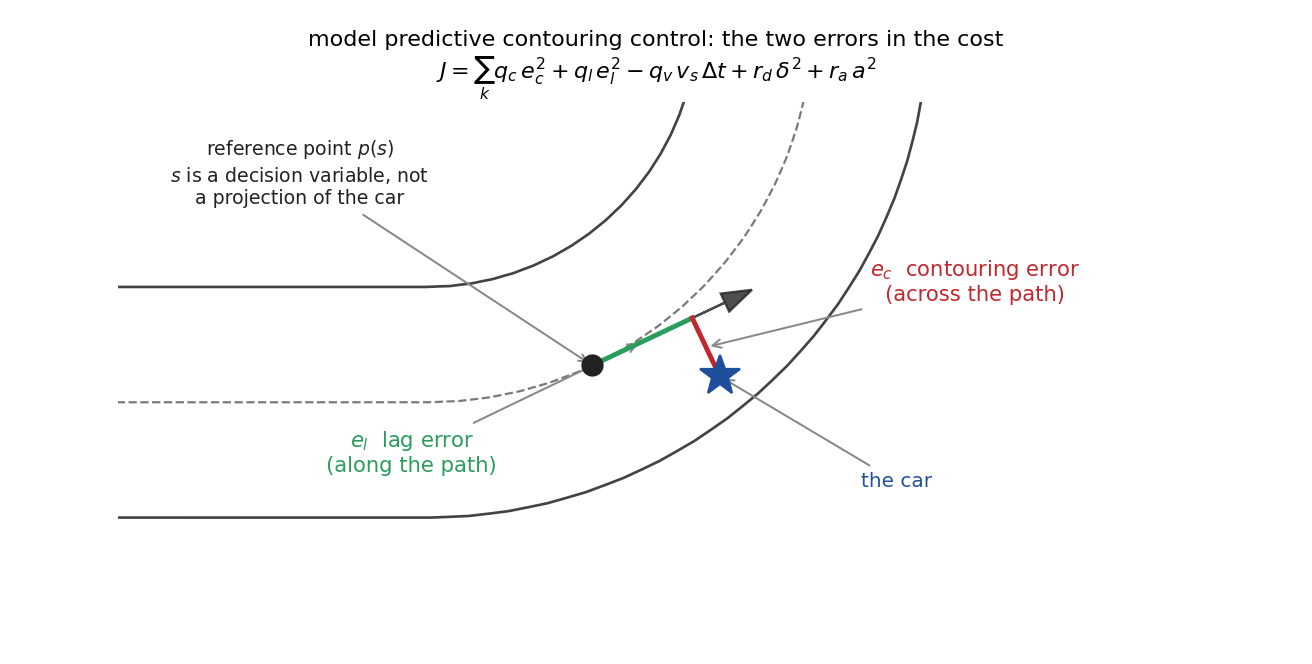
\includegraphics[width=\columnwidth]{figures/mpcc_geometry.png}
  \caption{Model predictive contouring control tracks a \emph{path} and carries
  its own progress $s$ as a decision variable. The reference point $p(s)$ is
  therefore chosen by the solver, not obtained by projection, and the vector to
  the car splits into a contouring error $e_c$ across the path and a lag error
  $e_l$ along it. Without a penalty on $e_l$ the cheapest way to collect the
  progress reward is to run $s$ forward and leave the car behind.}
  \label{fig:geometry}
\end{figure}

The cost, with $\theta = \log(q_c, q_l, q_v, r_\delta, r_a, r_{\dot s})$ the
learnable weights,
\begin{equation}
  J = \sum_k q_c e_c^2 + q_l e_l^2 - q_v \dot s\,\Delta t
      + r_\delta \delta^2 + r_a a^2 + r_{\dot s}(\dot s - v)^2 .
  \label{eq:cost}
\end{equation}

\section{Warm starts are memory}\label{sec:theory}

Write one solver tick as
\begin{equation}
  w_{t+1} = \Phi(w_t, s_t, \theta), \qquad u_t = g(w_t),
  \label{eq:phi}
\end{equation}
with $w$ the primal--dual iterate, $\Phi$ one RTI/SQP step and $g$ the
projection onto the first control. Compare a recurrent network,
$h_{t+1} = F(h_t, x_t, \theta)$. \emph{They are the same object}: the solver is
a recurrent cell whose update happens to be a Newton step. The influence
therefore obeys the recursion real-time recurrent learning uses,
\begin{equation}
  J_{t+1} = \underbrace{\frac{\partial\Phi}{\partial w}}_{D_t} J_t
            + \frac{\partial\Phi}{\partial\theta},
  \qquad J_t = \frac{\partial w_t}{\partial\theta},
  \label{eq:rtrl}
\end{equation}
and the sensitivity a policy-gradient update needs is
$\partial u_t/\partial\theta = (\partial g/\partial w)\,J_t$.

The envelope theorem is the $J_t \to$ fixed-point limit of
\eqref{eq:rtrl}: it is what \eqref{eq:phi} converges to when $\Phi$ is iterated
to convergence at every tick, so that $w_t$ carries no information about the
past. Because $D_t$ is the Jacobian of a contracting Newton map, $\|J_t\|$
loses history geometrically at rate $\rho(D)$, which is what makes a truncated
version of \eqref{eq:rtrl} affordable --- the same argument that justifies
truncation in RTRL.

\section{How wrong is the memoryless gradient?}\label{sec:rti}

\begin{figure*}[t]
  \centering
  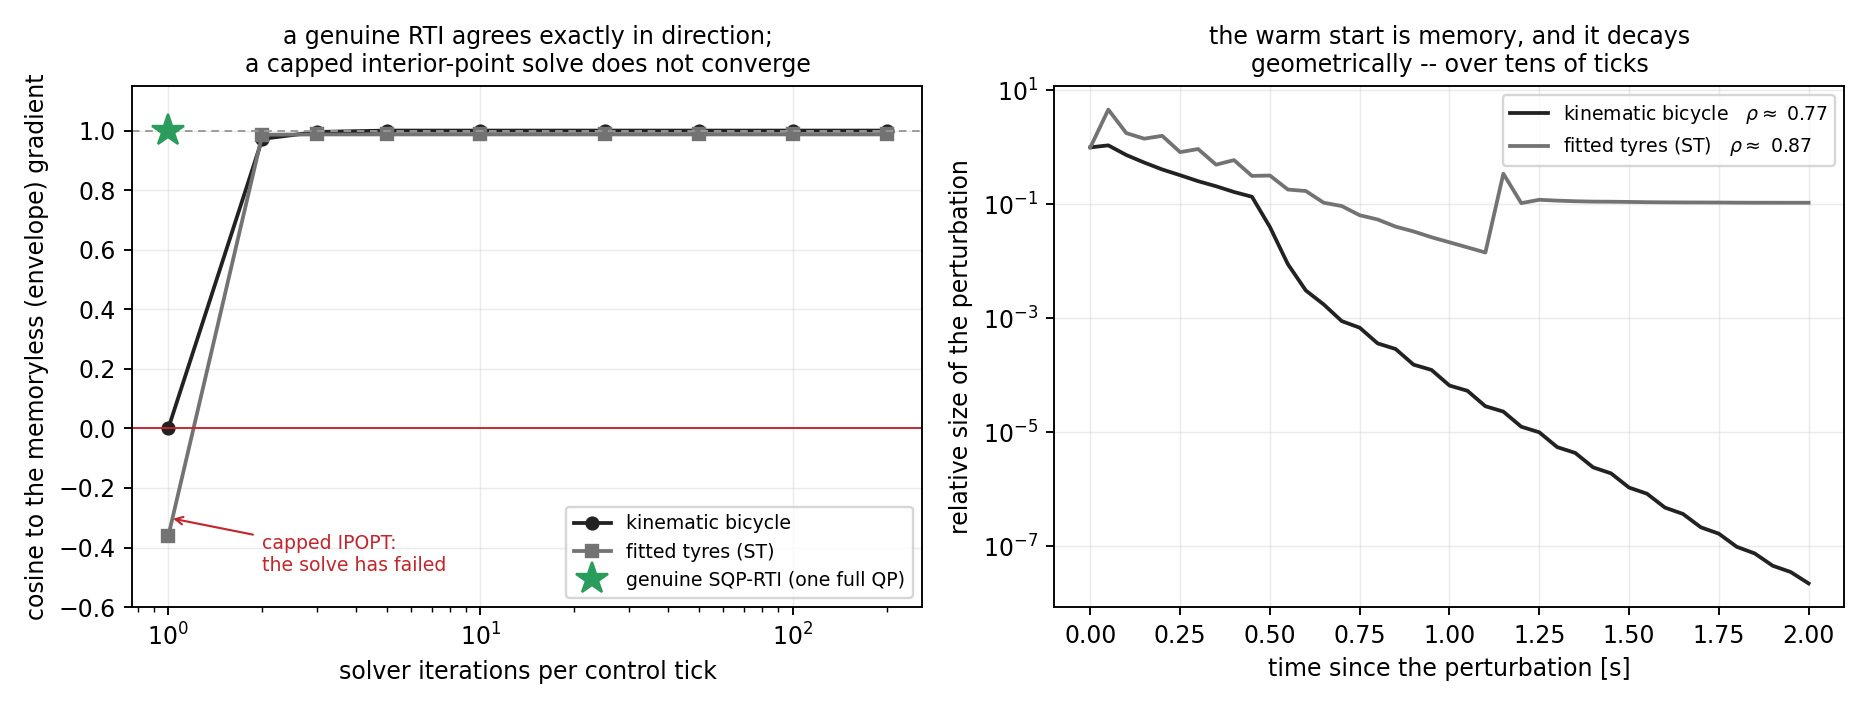
\includegraphics[width=\textwidth]{figures/rti_influence.png}
  \caption{\textbf{Left:} agreement between the sensitivity computed through the
  warm-started loop and the memoryless one, against solver effort. The point at
  one iteration is an interior-point solve that has \emph{failed}, not a
  real-time iteration; see Section~\ref{sec:trap}. \textbf{Right:} a
  perturbation of the warm start decays geometrically at $\rho \approx 0.77$
  and $0.87$. The warm start is genuinely memory --- it is simply not memory
  that reaches the gradient.
  Reproduced by \texttt{experiments/rti\_influence.py}.}
  \label{fig:rti}
\end{figure*}

\subsection{Isolating the solver}
Perturbing $\theta$ and running the closed loop conflates the solver's memory
with the fact that a different $\theta$ drives the car somewhere else. We
therefore \emph{replay} a recorded state sequence, so the only path from
$\theta$ to the iterate at tick $T$ is the chain of warm starts.

\subsection{Result}
Table~\ref{tab:rti}. With a genuine real-time iteration --- one full QP per
tick, warm-started, as in \texttt{acados}'s \textsc{sqp\_rti} --- the
sensitivity is \emph{identical in direction} to the memoryless one and $16\%$
smaller in magnitude. One QP step from a good warm start lands very close to
the converged solution: the mean step is $\lVert\Delta w\rVert = 0.748$ against
a converged step of $0.748$.

\begin{table}[t]
  \centering
  \caption{Sensitivity of the applied input to the cost weights, obtained three
  ways, on a replayed state sequence.}
  \label{tab:rti}
  \begin{tabular}{lrr}
    \toprule
    & $\lVert J\rVert$ & cosine to memoryless \\
    \midrule
    SQP-RTI, one QP, warm-started & 1.681 & \textbf{1.0000} \\
    warm-started \emph{and} converged & 1.994 & 1.0000 \\
    memoryless (cold, converged) & 1.994 & --- \\
    \bottomrule
  \end{tabular}
\end{table}

The recursion of Section~\ref{sec:theory} is a correct description of the
solver; the warm start really is state, and it really does decay geometrically
(Fig.~\ref{fig:rti}, right). The component of it that reaches
$\partial u_0/\partial\theta$ is simply small.

\subsection{The conclusion, stated as an assumption}
\begin{quote}\itshape
Differentiating a model-predictive controller as though it were converged is
justified for real-time iteration. This is an assumption the online-tuning
literature makes without stating; it holds, and the margin is $16\%$ in
magnitude and nothing in direction.
\end{quote}

\section{The test that says otherwise}\label{sec:trap}

There is an obvious way to approximate real-time iteration --- cap an
interior-point solver at one iteration --- and it gives the opposite answer.
Under that substitution the gradient appears \emph{orthogonal} to the
memoryless one, $\cos = 0.001$ on the kinematic bicycle and $-0.36$ on the
fitted-tyre plant, which reads as a decisive confirmation that solver memory
matters.

It is not. Those solves have failed:
\begin{itemize}
  \item $0$ of $41$ report success;
  \item the iterate moves by $8.19$ on average, an order of magnitude
        \emph{further} than a converged step ($0.748$), because an
        interior-point method's first step from a warm start is large and not
        yet meaningful.
\end{itemize}
The measured quantity is the parameter-sensitivity of a non-solution. Real-time
iteration is an SQP scheme --- linearise once, solve one full QP --- and the
distinction inverts the result. We report this because the wrong experiment is
cheaper and more natural than the right one, and because we ran it first.

\section{Surviving your own tuning}\label{sec:safety}

Unconstrained online tuning destroys the controller. From the paper's
initialisation the tuner improves the distance covered for five episodes
($73 \to 79$\,m) and then leaves the track on every subsequent episode, with
$q_c$ --- the weight holding the car near the path --- falling from $10$ to
$0.41$. Most of the damage occurs in episode~0, in which $q_v$ moves by a factor
of $222$.

A predictive safety filter removes the failure without touching the learner.

\begin{table}[t]
  \centering
  \caption{Online tuning with and without a predictive safety filter, same seed,
  26 episodes.}
  \label{tab:safety}
  \begin{tabular}{lrr}
    \toprule
     & no filter & with filter \\
    \midrule
    last 8 episodes, mean distance & \SI{7.6}{\meter} & \SI{68.1}{\meter} \\
    last 8 episodes, off-track     & 8 / 8 & \textbf{0 / 8} \\
    steps overridden, episodes 0--3 & --- & $0\%$ \\
    \bottomrule
  \end{tabular}
\end{table}

Two honest qualifications. The filter is \emph{invisible} until it is needed:
episodes 0--3 are bit-identical to the unfiltered run. But it converts a crash
into a slow degradation rather than preventing the degradation --- $q_c$ still
falls to $0.14$ by episode~20 --- because the consequence of pushing it down is
absorbed by the filter and never reaches the return. Evaluating the resulting
weights \emph{without} the filter gives the same distance as with it, so the
tuner did not learn to depend on the filter; it simply drifted.

\section{Real vehicle}\label{sec:real}
\todo{Not done. The controller does not yet survive the fitted-tyre plant from
the default initialisation: an open-loop sweep shows the feasible region exists
(every run with $r_\delta = 10$ completes 400 steps, every run with
$r_\delta = 1$ crashes) but the tuner overshoots it. Without either this or a
hardware result the paper is a negative result plus a measurement.}

\section{Conclusion}

A deployed MPC is formally a recurrent system, and we expected its gradient with
respect to its own cost weights to differ from the one the envelope theorem
provides. It does not, to any degree that matters: for real-time iteration the
direction is exact and the magnitude is $16\%$ low. The contribution is
therefore a negative one --- an assumption the field relies on silently, checked
and found sound --- together with a warning about the substitution that makes it
look unsound, and a safety filter that makes online tuning survivable in the
first place.

\bibliographystyle{IEEEtran}
\bibliography{refs}
\end{document}
